\documentclass[12pt,letterpaper]{article}
\usepackage{natbib}

%Packages
\usepackage{pdflscape}
\usepackage{fixltx2e}
\usepackage{textcomp}
\usepackage{fullpage}
\usepackage{float}
\usepackage{latexsym}
\usepackage{url}
\usepackage{epsfig}
\usepackage{graphicx}
\usepackage{amssymb}
\usepackage{amsmath}
\usepackage{mathtools}
\usepackage{bm}
\usepackage{array}
\usepackage[version=3]{mhchem}
\usepackage{ifthen}
\usepackage{caption}
\usepackage{hyperref}
\usepackage{amsthm}
\usepackage{amstext}
\usepackage{enumerate}
\usepackage[osf]{mathpazo}
\usepackage{dcolumn}
\usepackage{lineno}
\usepackage{dcolumn}
\usepackage{mathtools}
\usepackage{longtable}

\DeclarePairedDelimiter\abs{\lvert}{\rvert}%
\DeclarePairedDelimiter\norm{\lVert}{\rVert}%
\newcolumntype{d}[1]{D{.}{.}{#1}}

\pagenumbering{arabic}


%Pagination style and stuff
\linespread{2}
\raggedright
\setlength{\parindent}{0.5in}
\setcounter{secnumdepth}{0} 
\renewcommand{\section}[1]{%
\bigskip
\begin{center}
\begin{Large}
\normalfont\scshape #1
\medskip
\end{Large}
\end{center}}
\renewcommand{\subsection}[1]{%
\bigskip
\begin{center}
\begin{large}
\normalfont\itshape #1
\end{large}
\end{center}}
\renewcommand{\subsection}[1]{%
\vspace{2ex}
\noindent
\textit{#1.}---}
\renewcommand{\tableofcontents}{}
%\bibpunct{(}{)}{;}{a}{}{,}

%---------------------------------------------
%
%       START
%
%---------------------------------------------

\begin{document}

%Running head
\begin{flushright}
Version dated: \today
\end{flushright}
\bigskip
\noindent RH: Characters correlation

\bigskip
\medskip
\begin{center}

\noindent{\Large \bf Effect of discrete character correlation on tree inference}
\noindent{\Large \bf Supplementary material 3 - Additional results}
\bigskip

\noindent {\normalsize \sc Thomas Guillerme$^1$$^*$, and Martin D. Brazeau$^1$}\\
\noindent {\small \it 
$^1$Imperial College London, Silwood Park Campus, Department of Life Sciences, Buckhurst Road, Ascot SL5 7PY, United Kingdom.\\}
\end{center}
\medskip
\noindent{*\bf Corresponding author.} \textit{t.guillerme@imperial.ac.uk}\\ 

%Line numbering
% \modulolinenumbers[1]
% \linenumbers


\section{Signal to noise ratio}


\begin{figure}[!htbp]
\centering
   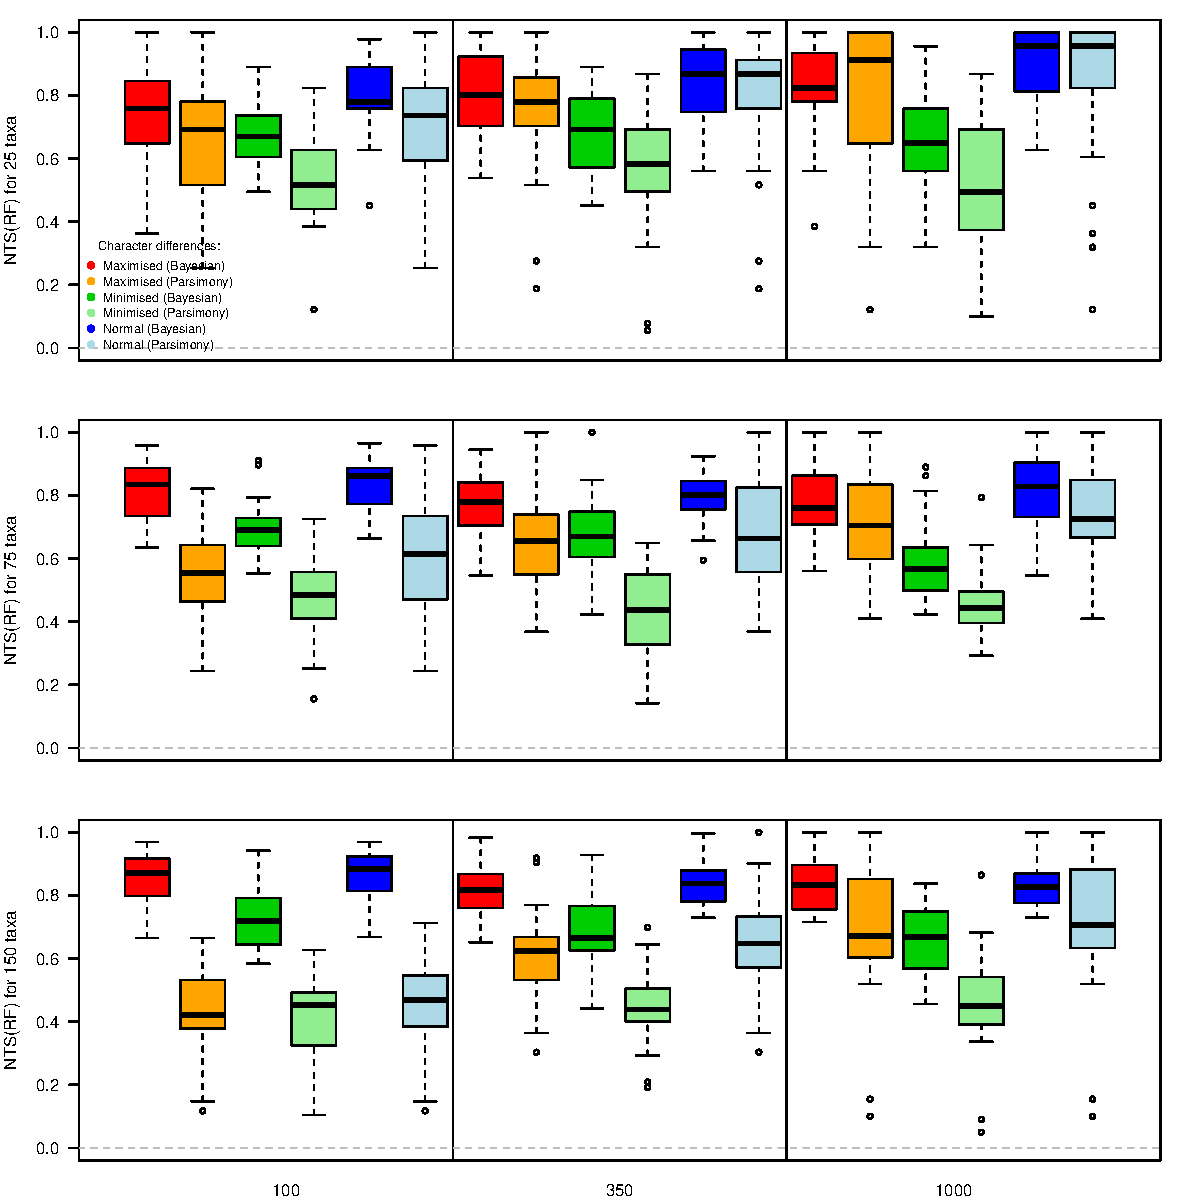
\includegraphics[width=1\textwidth]{../Figures/RF_results_null.pdf} %TG: These figures will be cleaned up once I have the final results.
\caption{Effect of Character Difference on recovering the ``random'' topology. The y axis represents the Normalised Tree Similarity using Robinson-Fould distance for matrices with 25, 75 and 150 taxa from top to bottom respectively. The x axis represents the different Character Difference scenarios and tree inference method with the Maximised Character Difference in Bayesian (red) and under Maximum Parsimony (orange), the Minimised Character Difference in Bayesian (dark green) and under Maximum Parsimony (light green) and the Randomised Character Difference in Bayesian (dark blue) and under Maximum Parsimony (light blue) for matrices of 100, 350 and 1000 characters in the panels from left to right.}
\label{Fig:RF_results_rand}
\end{figure}


\begin{figure}[!htbp]
\centering
   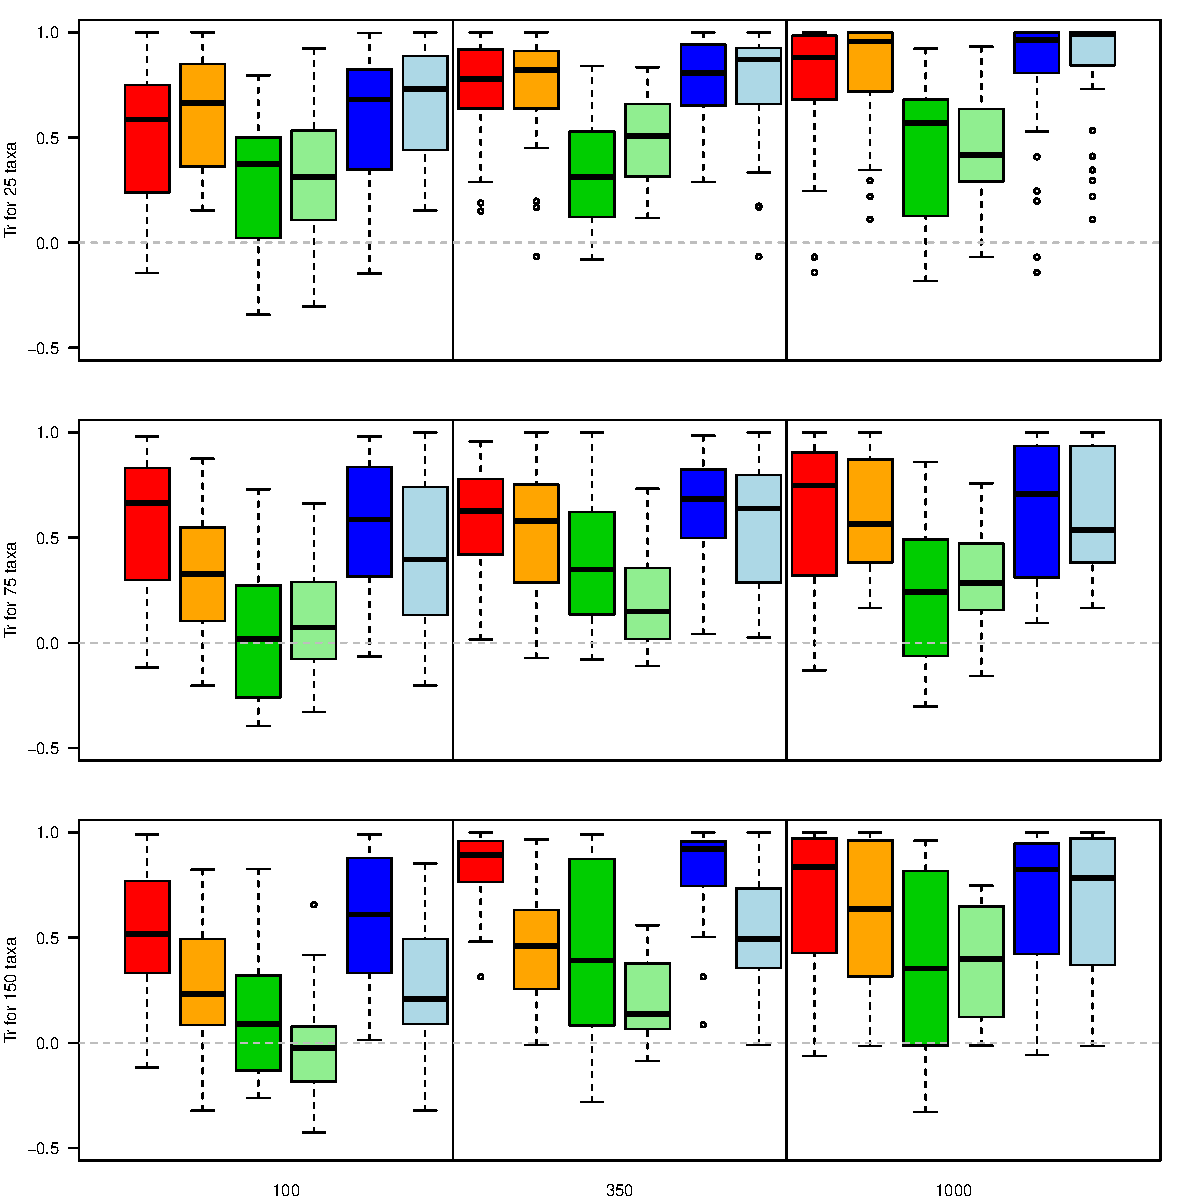
\includegraphics[width=1\textwidth]{../Figures/Tr_results_null.pdf} %TG: These figures will be cleaned up once I have the final results.
\caption{Effect of Character Difference on recovering the ``random'' topology. The axis are identical to figure \ref{Fig:RF_results_rand} but y axis represents the Normalised Tree Similarity using Triplets distance.}
\label{Fig:Tr_results_rand}
\end{figure}






\begin{longtable}{rllllrrrrrr}
\caption{Summary of the $NTS_{RF}$ when comparing to the normalised tree}\\

  \hline
 & V1 & V2 & V3 & V4 & Min. & 1st Qu. & Median & Mean & 3rd Qu. & Max. \\ 
  \hline
1 & t25 & c100 & bayesian & maxi & 0.56 & 0.78 & 0.87 & 0.86 & 0.96 & 1.00 \\ 
  2 & t25 & c100 & parsimony & mini & 0.45 & 0.65 & 0.69 & 0.71 & 0.80 & 0.87 \\ 
  3 & t25 & c100 & bayesian & rand & 0.45 & 0.76 & 0.80 & 0.82 & 0.91 & 0.98 \\ 
  4 & t25 & c100 & parsimony & maxi & 0.52 & 0.73 & 0.80 & 0.81 & 0.92 & 1.00 \\ 
  5 & t25 & c100 & bayesian & mini & 0.12 & 0.49 & 0.54 & 0.56 & 0.68 & 0.82 \\ 
  6 & t25 & c100 & parsimony & rand & 0.25 & 0.64 & 0.78 & 0.74 & 0.87 & 1.00 \\ 
  7 & t25 & c350 & bayesian & maxi & 0.54 & 0.74 & 0.89 & 0.84 & 0.98 & 1.00 \\ 
  8 & t25 & c350 & parsimony & mini & 0.41 & 0.56 & 0.74 & 0.69 & 0.79 & 0.93 \\ 
  9 & t25 & c350 & bayesian & rand & 0.56 & 0.75 & 0.88 & 0.84 & 0.96 & 1.00 \\ 
  10 & t25 & c350 & parsimony & maxi & 0.65 & 0.82 & 0.91 & 0.90 & 1.00 & 1.00 \\ 
  11 & t25 & c350 & bayesian & mini & 0.08 & 0.43 & 0.57 & 0.53 & 0.66 & 0.87 \\ 
  12 & t25 & c350 & parsimony & rand & 0.19 & 0.74 & 0.78 & 0.77 & 0.91 & 1.00 \\ 
  13 & t25 & c1000 & bayesian & maxi & 0.41 & 0.86 & 0.93 & 0.90 & 1.00 & 1.00 \\ 
  14 & t25 & c1000 & parsimony & mini & 0.21 & 0.56 & 0.69 & 0.68 & 0.79 & 0.96 \\ 
  15 & t25 & c1000 & bayesian & rand & 0.63 & 0.79 & 0.96 & 0.89 & 1.00 & 1.00 \\ 
  16 & t25 & c1000 & parsimony & maxi & 0.60 & 0.94 & 1.00 & 0.94 & 1.00 & 1.00 \\ 
  17 & t25 & c1000 & bayesian & mini & 0.14 & 0.33 & 0.45 & 0.49 & 0.69 & 0.91 \\ 
  18 & t25 & c1000 & parsimony & rand & 0.12 & 0.72 & 0.91 & 0.80 & 0.97 & 1.00 \\ 
  19 & t75 & c100 & bayesian & maxi & 0.65 & 0.85 & 0.98 & 0.92 & 0.99 & 1.00 \\ 
  20 & t75 & c100 & parsimony & mini & 0.55 & 0.64 & 0.72 & 0.71 & 0.78 & 0.94 \\ 
  21 & t75 & c100 & bayesian & rand & 0.66 & 0.77 & 0.86 & 0.84 & 0.88 & 0.98 \\ 
  22 & t75 & c100 & parsimony & maxi & 0.49 & 0.75 & 1.00 & 0.88 & 1.00 & 1.00 \\ 
  23 & t75 & c100 & bayesian & mini & 0.21 & 0.41 & 0.46 & 0.47 & 0.54 & 0.88 \\ 
  24 & t75 & c100 & parsimony & rand & 0.24 & 0.43 & 0.52 & 0.55 & 0.67 & 0.96 \\ 
  25 & t75 & c350 & bayesian & maxi & 0.57 & 0.86 & 0.95 & 0.91 & 0.99 & 1.00 \\ 
  26 & t75 & c350 & parsimony & mini & 0.40 & 0.61 & 0.70 & 0.69 & 0.77 & 0.86 \\ 
  27 & t75 & c350 & bayesian & rand & 0.66 & 0.77 & 0.81 & 0.81 & 0.85 & 0.99 \\ 
  28 & t75 & c350 & parsimony & maxi & 0.61 & 0.78 & 0.99 & 0.89 & 1.00 & 1.00 \\ 
  29 & t75 & c350 & bayesian & mini & 0.22 & 0.32 & 0.40 & 0.42 & 0.50 & 0.72 \\ 
  30 & t75 & c350 & parsimony & rand & 0.37 & 0.55 & 0.66 & 0.69 & 0.87 & 1.00 \\ 
  31 & t75 & c1000 & bayesian & maxi & 0.57 & 0.83 & 0.90 & 0.90 & 0.98 & 1.00 \\ 
  32 & t75 & c1000 & parsimony & mini & 0.43 & 0.47 & 0.59 & 0.62 & 0.70 & 0.94 \\ 
  33 & t75 & c1000 & bayesian & rand & 0.55 & 0.71 & 0.81 & 0.78 & 0.87 & 0.99 \\ 
  34 & t75 & c1000 & parsimony & maxi & 0.55 & 1.00 & 1.00 & 0.95 & 1.00 & 1.00 \\ 
  35 & t75 & c1000 & bayesian & mini & 0.28 & 0.42 & 0.44 & 0.48 & 0.48 & 0.89 \\ 
  36 & t75 & c1000 & parsimony & rand & 0.41 & 0.67 & 0.69 & 0.70 & 0.77 & 0.94 \\ 
  37 & t150 & c100 & bayesian & maxi & 0.95 & 0.98 & 0.99 & 0.99 & 1.00 & 1.00 \\ 
  38 & t150 & c100 & parsimony & mini & 0.60 & 0.74 & 0.76 & 0.77 & 0.81 & 0.89 \\ 
  39 & t150 & c100 & bayesian & rand & 0.76 & 0.84 & 0.90 & 0.88 & 0.92 & 0.94 \\ 
  40 & t150 & c100 & parsimony & maxi & 0.50 & 0.57 & 0.78 & 0.78 & 1.00 & 1.00 \\ 
  41 & t150 & c100 & bayesian & mini & 0.15 & 0.43 & 0.47 & 0.46 & 0.54 & 0.68 \\ 
  42 & t150 & c100 & parsimony & rand & 0.15 & 0.38 & 0.48 & 0.46 & 0.54 & 0.71 \\ 
  43 & t150 & c350 & bayesian & maxi & 0.92 & 0.97 & 0.98 & 0.97 & 0.99 & 1.00 \\ 
  44 & t150 & c350 & parsimony & mini & 0.62 & 0.66 & 0.68 & 0.71 & 0.75 & 0.89 \\ 
  45 & t150 & c350 & bayesian & rand & 0.73 & 0.77 & 0.81 & 0.81 & 0.85 & 0.90 \\ 
  46 & t150 & c350 & parsimony & maxi & 0.57 & 0.69 & 0.91 & 0.85 & 1.00 & 1.00 \\ 
  47 & t150 & c350 & bayesian & mini & 0.23 & 0.36 & 0.43 & 0.44 & 0.52 & 0.74 \\ 
  48 & t150 & c350 & parsimony & rand & 0.36 & 0.54 & 0.62 & 0.61 & 0.67 & 0.78 \\ 
  49 & t150 & c1000 & bayesian & maxi & 0.83 & 0.98 & 0.99 & 0.97 & 0.99 & 1.00 \\ 
  50 & t150 & c1000 & parsimony & mini & 0.49 & 0.57 & 0.59 & 0.59 & 0.62 & 0.67 \\ 
  51 & t150 & c1000 & bayesian & rand & 0.74 & 0.77 & 0.80 & 0.80 & 0.82 & 0.88 \\ 
  52 & t150 & c1000 & parsimony & maxi & 0.73 & 0.85 & 0.97 & 0.92 & 1.00 & 1.00 \\ 
  53 & t150 & c1000 & bayesian & mini & 0.11 & 0.41 & 0.45 & 0.44 & 0.50 & 0.61 \\ 
  54 & t150 & c1000 & parsimony & rand & 0.15 & 0.63 & 0.76 & 0.73 & 0.90 & 1.00 \\ 
   \hline
\end{longtable}


\begin{longtable}{rllllrrrrrr}
\caption{Summary of the $NTS_{RF}$ when comparing to the normalised tree}\\

  \hline
 & V1 & V2 & V3 & V4 & Min. & 1st Qu. & Median & Mean & 3rd Qu. & Max. \\ 
  \hline
1 & t25 & c100 & bayesian & maxi & -0.01 & 0.63 & 0.84 & 0.76 & 0.97 & 1.00 \\ 
  2 & t25 & c100 & parsimony & mini & -0.39 & 0.09 & 0.37 & 0.34 & 0.60 & 0.84 \\ 
  3 & t25 & c100 & bayesian & rand & -0.15 & 0.49 & 0.71 & 0.64 & 0.83 & 1.00 \\ 
  4 & t25 & c100 & parsimony & maxi & 0.24 & 0.76 & 0.95 & 0.85 & 0.98 & 1.00 \\ 
  5 & t25 & c100 & bayesian & mini & -0.13 & 0.29 & 0.55 & 0.51 & 0.76 & 0.92 \\ 
  6 & t25 & c100 & parsimony & rand & 0.15 & 0.73 & 0.87 & 0.79 & 0.96 & 1.00 \\ 
  7 & t25 & c350 & bayesian & maxi & 0.18 & 0.73 & 0.92 & 0.84 & 0.98 & 1.00 \\ 
  8 & t25 & c350 & parsimony & mini & -0.18 & 0.07 & 0.35 & 0.35 & 0.60 & 0.87 \\ 
  9 & t25 & c350 & bayesian & rand & 0.29 & 0.67 & 0.82 & 0.78 & 0.96 & 1.00 \\ 
  10 & t25 & c350 & parsimony & maxi & 0.33 & 0.82 & 0.97 & 0.88 & 1.00 & 1.00 \\ 
  11 & t25 & c350 & bayesian & mini & -0.01 & 0.24 & 0.47 & 0.44 & 0.61 & 0.89 \\ 
  12 & t25 & c350 & parsimony & rand & -0.07 & 0.69 & 0.88 & 0.73 & 0.93 & 1.00 \\ 
  13 & t25 & c1000 & bayesian & maxi & 0.37 & 0.83 & 0.98 & 0.90 & 1.00 & 1.00 \\ 
  14 & t25 & c1000 & parsimony & mini & -0.21 & 0.16 & 0.53 & 0.47 & 0.72 & 0.92 \\ 
  15 & t25 & c1000 & bayesian & rand & -0.14 & 0.80 & 0.94 & 0.81 & 1.00 & 1.00 \\ 
  16 & t25 & c1000 & parsimony & maxi & 0.54 & 0.99 & 1.00 & 0.95 & 1.00 & 1.00 \\ 
  17 & t25 & c1000 & bayesian & mini & -0.06 & 0.20 & 0.35 & 0.39 & 0.62 & 0.93 \\ 
  18 & t25 & c1000 & parsimony & rand & 0.22 & 0.68 & 0.96 & 0.80 & 1.00 & 1.00 \\ 
  19 & t75 & c100 & bayesian & maxi & 0.00 & 0.61 & 0.96 & 0.79 & 1.00 & 1.00 \\ 
  20 & t75 & c100 & parsimony & mini & -0.47 & -0.27 & -0.02 & 0.07 & 0.42 & 0.90 \\ 
  21 & t75 & c100 & bayesian & rand & -0.07 & 0.32 & 0.68 & 0.55 & 0.82 & 0.98 \\ 
  22 & t75 & c100 & parsimony & maxi & 0.22 & 0.81 & 1.00 & 0.85 & 1.00 & 1.00 \\ 
  23 & t75 & c100 & bayesian & mini & -0.34 & -0.09 & -0.02 & 0.06 & 0.11 & 0.83 \\ 
  24 & t75 & c100 & parsimony & rand & -0.20 & 0.10 & 0.35 & 0.36 & 0.55 & 1.00 \\ 
  25 & t75 & c350 & bayesian & maxi & 0.14 & 0.79 & 0.94 & 0.85 & 0.99 & 1.00 \\ 
  26 & t75 & c350 & parsimony & mini & -0.31 & 0.22 & 0.43 & 0.41 & 0.68 & 0.93 \\ 
  27 & t75 & c350 & bayesian & rand & 0.04 & 0.56 & 0.72 & 0.65 & 0.84 & 1.00 \\ 
  28 & t75 & c350 & parsimony & maxi & 0.30 & 0.73 & 1.00 & 0.84 & 1.00 & 1.00 \\ 
  29 & t75 & c350 & bayesian & mini & -0.06 & 0.10 & 0.17 & 0.23 & 0.37 & 0.73 \\ 
  30 & t75 & c350 & parsimony & rand & 0.03 & 0.30 & 0.69 & 0.61 & 0.92 & 1.00 \\ 
  31 & t75 & c1000 & bayesian & maxi & 0.23 & 0.59 & 0.85 & 0.76 & 1.00 & 1.00 \\ 
  32 & t75 & c1000 & parsimony & mini & -0.20 & -0.07 & 0.10 & 0.28 & 0.67 & 0.86 \\ 
  33 & t75 & c1000 & bayesian & rand & 0.10 & 0.30 & 0.45 & 0.51 & 0.83 & 1.00 \\ 
  34 & t75 & c1000 & parsimony & maxi & 0.52 & 1.00 & 1.00 & 0.94 & 1.00 & 1.00 \\ 
  35 & t75 & c1000 & bayesian & mini & -0.00 & 0.11 & 0.22 & 0.29 & 0.39 & 0.85 \\ 
  36 & t75 & c1000 & parsimony & rand & 0.17 & 0.34 & 0.49 & 0.49 & 0.58 & 0.94 \\ 
  37 & t150 & c100 & bayesian & maxi & 0.52 & 1.00 & 1.00 & 0.96 & 1.00 & 1.00 \\ 
  38 & t150 & c100 & parsimony & mini & -0.30 & -0.16 & -0.01 & 0.08 & 0.21 & 0.67 \\ 
  39 & t150 & c100 & bayesian & rand & 0.01 & 0.32 & 0.58 & 0.61 & 0.96 & 0.99 \\ 
  40 & t150 & c100 & parsimony & maxi & -0.03 & 0.44 & 0.69 & 0.66 & 1.00 & 1.00 \\ 
  41 & t150 & c100 & bayesian & mini & -0.42 & -0.20 & 0.01 & -0.03 & 0.12 & 0.32 \\ 
  42 & t150 & c100 & parsimony & rand & -0.32 & 0.10 & 0.20 & 0.24 & 0.48 & 0.64 \\ 
  43 & t150 & c350 & bayesian & maxi & 0.60 & 0.98 & 0.99 & 0.97 & 1.00 & 1.00 \\ 
  44 & t150 & c350 & parsimony & mini & -0.11 & 0.46 & 0.76 & 0.64 & 0.91 & 0.98 \\ 
  45 & t150 & c350 & bayesian & rand & 0.53 & 0.83 & 0.93 & 0.87 & 0.96 & 0.98 \\ 
  46 & t150 & c350 & parsimony & maxi & 0.31 & 0.72 & 0.91 & 0.81 & 1.00 & 1.00 \\ 
  47 & t150 & c350 & bayesian & mini & -0.05 & -0.01 & 0.10 & 0.17 & 0.33 & 0.59 \\ 
  48 & t150 & c350 & parsimony & rand & 0.08 & 0.32 & 0.48 & 0.44 & 0.53 & 0.81 \\ 
  49 & t150 & c1000 & bayesian & maxi & 0.05 & 0.50 & 0.85 & 0.70 & 0.97 & 0.99 \\ 
  50 & t150 & c1000 & parsimony & mini & -0.21 & -0.04 & 0.14 & 0.19 & 0.33 & 0.83 \\ 
  51 & t150 & c1000 & bayesian & rand & -0.06 & 0.21 & 0.38 & 0.42 & 0.67 & 0.91 \\ 
  52 & t150 & c1000 & parsimony & maxi & 0.50 & 0.88 & 1.00 & 0.92 & 1.00 & 1.00 \\ 
  53 & t150 & c1000 & bayesian & mini & 0.04 & 0.11 & 0.29 & 0.36 & 0.60 & 0.72 \\ 
  54 & t150 & c1000 & parsimony & rand & 0.03 & 0.46 & 0.80 & 0.70 & 0.97 & 1.00 \\ 
   \hline
\end{longtable}


\begin{longtable}{rllllrrrrrr}
\caption{Summary of the $NTS_{RF}$ when comparing to the normalised tree}\\

  \hline
 & V1 & V2 & V3 & V4 & Min. & 1st Qu. & Median & Mean & 3rd Qu. & Max. \\ 
  \hline
1 & t25 & c100 & bayesian & norm & 0.45 & 0.76 & 0.80 & 0.82 & 0.91 & 0.98 \\ 
  2 & t25 & c100 & parsimony & maxi & 0.36 & 0.65 & 0.78 & 0.76 & 0.87 & 1.00 \\ 
  3 & t25 & c100 & bayesian & mini & 0.49 & 0.60 & 0.67 & 0.66 & 0.74 & 0.89 \\ 
  4 & t25 & c100 & parsimony & norm & 0.25 & 0.64 & 0.78 & 0.74 & 0.87 & 1.00 \\ 
  5 & t25 & c100 & bayesian & maxi & 0.25 & 0.54 & 0.74 & 0.69 & 0.81 & 1.00 \\ 
  6 & t25 & c100 & parsimony & mini & 0.12 & 0.42 & 0.48 & 0.51 & 0.61 & 0.82 \\ 
  7 & t25 & c350 & bayesian & norm & 0.56 & 0.75 & 0.88 & 0.84 & 0.96 & 1.00 \\ 
  8 & t25 & c350 & parsimony & maxi & 0.54 & 0.72 & 0.80 & 0.81 & 0.93 & 1.00 \\ 
  9 & t25 & c350 & bayesian & mini & 0.45 & 0.58 & 0.69 & 0.67 & 0.78 & 0.89 \\ 
  10 & t25 & c350 & parsimony & norm & 0.19 & 0.74 & 0.78 & 0.77 & 0.91 & 1.00 \\ 
  11 & t25 & c350 & bayesian & maxi & 0.19 & 0.69 & 0.78 & 0.74 & 0.82 & 1.00 \\ 
  12 & t25 & c350 & parsimony & mini & 0.06 & 0.46 & 0.56 & 0.52 & 0.65 & 0.82 \\ 
  13 & t25 & c1000 & bayesian & norm & 0.63 & 0.79 & 0.96 & 0.89 & 1.00 & 1.00 \\ 
  14 & t25 & c1000 & parsimony & maxi & 0.39 & 0.72 & 0.82 & 0.82 & 0.93 & 1.00 \\ 
  15 & t25 & c1000 & bayesian & mini & 0.25 & 0.56 & 0.69 & 0.66 & 0.76 & 0.96 \\ 
  16 & t25 & c1000 & parsimony & norm & 0.12 & 0.72 & 0.91 & 0.80 & 0.97 & 1.00 \\ 
  17 & t25 & c1000 & bayesian & maxi & 0.12 & 0.60 & 0.85 & 0.75 & 0.97 & 1.00 \\ 
  18 & t25 & c1000 & parsimony & mini & 0.10 & 0.33 & 0.45 & 0.48 & 0.69 & 0.87 \\ 
  19 & t75 & c100 & bayesian & norm & 0.66 & 0.77 & 0.86 & 0.84 & 0.88 & 0.98 \\ 
  20 & t75 & c100 & parsimony & maxi & 0.64 & 0.73 & 0.82 & 0.81 & 0.88 & 0.96 \\ 
  21 & t75 & c100 & bayesian & mini & 0.55 & 0.63 & 0.68 & 0.69 & 0.73 & 0.91 \\ 
  22 & t75 & c100 & parsimony & norm & 0.24 & 0.43 & 0.52 & 0.55 & 0.67 & 0.96 \\ 
  23 & t75 & c100 & bayesian & maxi & 0.24 & 0.43 & 0.49 & 0.51 & 0.59 & 0.77 \\ 
  24 & t75 & c100 & parsimony & mini & 0.15 & 0.40 & 0.46 & 0.45 & 0.56 & 0.67 \\ 
  25 & t75 & c350 & bayesian & norm & 0.66 & 0.77 & 0.81 & 0.81 & 0.85 & 0.99 \\ 
  26 & t75 & c350 & parsimony & maxi & 0.55 & 0.72 & 0.78 & 0.78 & 0.84 & 0.98 \\ 
  27 & t75 & c350 & bayesian & mini & 0.42 & 0.61 & 0.70 & 0.67 & 0.75 & 0.85 \\ 
  28 & t75 & c350 & parsimony & norm & 0.37 & 0.55 & 0.66 & 0.69 & 0.87 & 1.00 \\ 
  29 & t75 & c350 & bayesian & maxi & 0.37 & 0.52 & 0.65 & 0.64 & 0.73 & 1.00 \\ 
  30 & t75 & c350 & parsimony & mini & 0.23 & 0.30 & 0.41 & 0.41 & 0.49 & 0.61 \\ 
  31 & t75 & c1000 & bayesian & norm & 0.55 & 0.71 & 0.81 & 0.78 & 0.87 & 0.99 \\ 
  32 & t75 & c1000 & parsimony & maxi & 0.56 & 0.70 & 0.75 & 0.74 & 0.81 & 0.97 \\ 
  33 & t75 & c1000 & bayesian & mini & 0.42 & 0.46 & 0.61 & 0.60 & 0.64 & 0.89 \\ 
  34 & t75 & c1000 & parsimony & norm & 0.41 & 0.67 & 0.69 & 0.70 & 0.77 & 0.94 \\ 
  35 & t75 & c1000 & bayesian & maxi & 0.41 & 0.64 & 0.69 & 0.68 & 0.75 & 0.95 \\ 
  36 & t75 & c1000 & parsimony & mini & 0.29 & 0.41 & 0.44 & 0.46 & 0.47 & 0.79 \\ 
  37 & t150 & c100 & bayesian & norm & 0.76 & 0.84 & 0.90 & 0.88 & 0.92 & 0.94 \\ 
  38 & t150 & c100 & parsimony & maxi & 0.76 & 0.83 & 0.90 & 0.88 & 0.93 & 0.94 \\ 
  39 & t150 & c100 & bayesian & mini & 0.59 & 0.70 & 0.77 & 0.76 & 0.81 & 0.87 \\ 
  40 & t150 & c100 & parsimony & norm & 0.15 & 0.38 & 0.48 & 0.46 & 0.54 & 0.71 \\ 
  41 & t150 & c100 & bayesian & maxi & 0.15 & 0.38 & 0.42 & 0.44 & 0.52 & 0.67 \\ 
  42 & t150 & c100 & parsimony & mini & 0.13 & 0.37 & 0.47 & 0.43 & 0.49 & 0.63 \\ 
  43 & t150 & c350 & bayesian & norm & 0.73 & 0.77 & 0.81 & 0.81 & 0.85 & 0.90 \\ 
  44 & t150 & c350 & parsimony & maxi & 0.74 & 0.76 & 0.80 & 0.81 & 0.86 & 0.91 \\ 
  45 & t150 & c350 & bayesian & mini & 0.58 & 0.65 & 0.71 & 0.73 & 0.77 & 0.93 \\ 
  46 & t150 & c350 & parsimony & norm & 0.36 & 0.54 & 0.62 & 0.61 & 0.67 & 0.78 \\ 
  47 & t150 & c350 & bayesian & maxi & 0.36 & 0.52 & 0.60 & 0.58 & 0.64 & 0.77 \\ 
  48 & t150 & c350 & parsimony & mini & 0.21 & 0.34 & 0.43 & 0.43 & 0.50 & 0.70 \\ 
  49 & t150 & c1000 & bayesian & norm & 0.74 & 0.77 & 0.80 & 0.80 & 0.82 & 0.88 \\ 
  50 & t150 & c1000 & parsimony & maxi & 0.73 & 0.76 & 0.79 & 0.79 & 0.82 & 0.88 \\ 
  51 & t150 & c1000 & bayesian & mini & 0.47 & 0.55 & 0.58 & 0.58 & 0.62 & 0.68 \\ 
  52 & t150 & c1000 & parsimony & norm & 0.15 & 0.63 & 0.76 & 0.73 & 0.90 & 1.00 \\ 
  53 & t150 & c1000 & bayesian & maxi & 0.15 & 0.62 & 0.71 & 0.73 & 0.96 & 1.00 \\ 
  54 & t150 & c1000 & parsimony & mini & 0.09 & 0.40 & 0.45 & 0.43 & 0.49 & 0.58 \\ 
   \hline
\end{longtable}



\begin{longtable}{rllllrrrrrr}
\caption{Summary of the $NTS_{RF}$ when comparing to the normalised tree}\\

  \hline
 & V1 & V2 & V3 & V4 & Min. & 1st Qu. & Median & Mean & 3rd Qu. & Max. \\ 
  \hline
1 & t25 & c100 & bayesian & norm & -0.15 & 0.49 & 0.71 & 0.64 & 0.83 & 1.00 \\ 
  2 & t25 & c100 & parsimony & maxi & -0.14 & 0.47 & 0.66 & 0.58 & 0.78 & 1.00 \\ 
  3 & t25 & c100 & bayesian & mini & -0.34 & 0.04 & 0.37 & 0.28 & 0.50 & 0.80 \\ 
  4 & t25 & c100 & parsimony & norm & 0.15 & 0.73 & 0.87 & 0.79 & 0.96 & 1.00 \\ 
  5 & t25 & c100 & bayesian & maxi & 0.15 & 0.50 & 0.80 & 0.71 & 0.95 & 1.00 \\ 
  6 & t25 & c100 & parsimony & mini & -0.11 & 0.30 & 0.52 & 0.47 & 0.61 & 0.92 \\ 
  7 & t25 & c350 & bayesian & norm & 0.29 & 0.67 & 0.82 & 0.78 & 0.96 & 1.00 \\ 
  8 & t25 & c350 & parsimony & maxi & 0.15 & 0.66 & 0.79 & 0.75 & 0.92 & 1.00 \\ 
  9 & t25 & c350 & bayesian & mini & -0.08 & 0.14 & 0.32 & 0.35 & 0.57 & 0.84 \\ 
  10 & t25 & c350 & parsimony & norm & -0.07 & 0.69 & 0.88 & 0.73 & 0.93 & 1.00 \\ 
  11 & t25 & c350 & bayesian & maxi & -0.07 & 0.61 & 0.87 & 0.71 & 0.91 & 1.00 \\ 
  12 & t25 & c350 & parsimony & mini & 0.12 & 0.31 & 0.52 & 0.49 & 0.66 & 0.83 \\ 
  13 & t25 & c1000 & bayesian & norm & -0.14 & 0.80 & 0.94 & 0.81 & 1.00 & 1.00 \\ 
  14 & t25 & c1000 & parsimony & maxi & -0.14 & 0.64 & 0.88 & 0.76 & 0.97 & 1.00 \\ 
  15 & t25 & c1000 & bayesian & mini & -0.18 & 0.09 & 0.53 & 0.42 & 0.68 & 0.92 \\ 
  16 & t25 & c1000 & parsimony & norm & 0.22 & 0.68 & 0.96 & 0.80 & 1.00 & 1.00 \\ 
  17 & t25 & c1000 & bayesian & maxi & 0.22 & 0.53 & 0.84 & 0.76 & 1.00 & 1.00 \\ 
  18 & t25 & c1000 & parsimony & mini & -0.07 & 0.26 & 0.37 & 0.42 & 0.62 & 0.85 \\ 
  19 & t75 & c100 & bayesian & norm & -0.07 & 0.32 & 0.68 & 0.55 & 0.82 & 0.98 \\ 
  20 & t75 & c100 & parsimony & maxi & -0.12 & 0.33 & 0.66 & 0.54 & 0.83 & 0.98 \\ 
  21 & t75 & c100 & bayesian & mini & -0.40 & -0.24 & 0.02 & 0.04 & 0.27 & 0.73 \\ 
  22 & t75 & c100 & parsimony & norm & -0.20 & 0.10 & 0.35 & 0.36 & 0.55 & 1.00 \\ 
  23 & t75 & c100 & bayesian & maxi & -0.20 & 0.10 & 0.28 & 0.32 & 0.52 & 0.88 \\ 
  24 & t75 & c100 & parsimony & mini & -0.33 & -0.04 & 0.06 & 0.10 & 0.18 & 0.66 \\ 
  25 & t75 & c350 & bayesian & norm & 0.04 & 0.56 & 0.72 & 0.65 & 0.84 & 1.00 \\ 
  26 & t75 & c350 & parsimony & maxi & 0.01 & 0.47 & 0.67 & 0.62 & 0.81 & 0.96 \\ 
  27 & t75 & c350 & bayesian & mini & -0.08 & 0.10 & 0.35 & 0.39 & 0.63 & 0.92 \\ 
  28 & t75 & c350 & parsimony & norm & 0.03 & 0.30 & 0.69 & 0.61 & 0.92 & 1.00 \\ 
  29 & t75 & c350 & bayesian & maxi & 0.03 & 0.29 & 0.59 & 0.51 & 0.71 & 1.00 \\ 
  30 & t75 & c350 & parsimony & mini & -0.11 & 0.01 & 0.15 & 0.21 & 0.42 & 0.73 \\ 
  31 & t75 & c1000 & bayesian & norm & 0.10 & 0.30 & 0.45 & 0.51 & 0.83 & 1.00 \\ 
  32 & t75 & c1000 & parsimony & maxi & -0.13 & 0.22 & 0.45 & 0.47 & 0.77 & 1.00 \\ 
  33 & t75 & c1000 & bayesian & mini & -0.30 & -0.08 & 0.24 & 0.21 & 0.47 & 0.86 \\ 
  34 & t75 & c1000 & parsimony & norm & 0.17 & 0.34 & 0.49 & 0.49 & 0.58 & 0.94 \\ 
  35 & t75 & c1000 & bayesian & maxi & 0.17 & 0.34 & 0.53 & 0.49 & 0.60 & 0.90 \\ 
  36 & t75 & c1000 & parsimony & mini & -0.16 & 0.14 & 0.27 & 0.26 & 0.36 & 0.76 \\ 
  37 & t150 & c100 & bayesian & norm & 0.01 & 0.32 & 0.58 & 0.61 & 0.96 & 0.99 \\ 
  38 & t150 & c100 & parsimony & maxi & 0.01 & 0.32 & 0.51 & 0.58 & 0.89 & 0.99 \\ 
  39 & t150 & c100 & bayesian & mini & -0.24 & -0.14 & -0.07 & 0.01 & 0.10 & 0.67 \\ 
  40 & t150 & c100 & parsimony & norm & -0.32 & 0.10 & 0.20 & 0.24 & 0.48 & 0.64 \\ 
  41 & t150 & c100 & bayesian & maxi & -0.32 & 0.09 & 0.22 & 0.27 & 0.55 & 0.71 \\ 
  42 & t150 & c100 & parsimony & mini & -0.43 & -0.20 & -0.04 & -0.06 & 0.07 & 0.42 \\ 
  43 & t150 & c350 & bayesian & norm & 0.53 & 0.83 & 0.93 & 0.87 & 0.96 & 0.98 \\ 
  44 & t150 & c350 & parsimony & maxi & 0.63 & 0.86 & 0.93 & 0.89 & 0.96 & 0.98 \\ 
  45 & t150 & c350 & bayesian & mini & -0.12 & 0.43 & 0.85 & 0.66 & 0.92 & 0.99 \\ 
  46 & t150 & c350 & parsimony & norm & 0.08 & 0.32 & 0.48 & 0.44 & 0.53 & 0.81 \\ 
  47 & t150 & c350 & bayesian & maxi & 0.08 & 0.31 & 0.46 & 0.45 & 0.59 & 0.81 \\ 
  48 & t150 & c350 & parsimony & mini & -0.09 & 0.03 & 0.13 & 0.18 & 0.32 & 0.56 \\ 
  49 & t150 & c1000 & bayesian & norm & -0.06 & 0.21 & 0.38 & 0.42 & 0.67 & 0.91 \\ 
  50 & t150 & c1000 & parsimony & maxi & -0.04 & 0.16 & 0.50 & 0.46 & 0.79 & 0.85 \\ 
  51 & t150 & c1000 & bayesian & mini & -0.21 & -0.10 & -0.02 & 0.13 & 0.15 & 0.88 \\ 
  52 & t150 & c1000 & parsimony & norm & 0.03 & 0.46 & 0.80 & 0.70 & 0.97 & 1.00 \\ 
  53 & t150 & c1000 & bayesian & maxi & 0.03 & 0.46 & 0.66 & 0.67 & 1.00 & 1.00 \\ 
  54 & t150 & c1000 & parsimony & mini & -0.01 & 0.13 & 0.29 & 0.37 & 0.64 & 0.75 \\ 
   \hline
\end{longtable}

\end{document}